\newif\ifQR
%\QRtrue
\QRfalse

\documentclass[uplatex,a4paper]{jsarticle}
\usepackage[at]{easylist} 
\usepackage{eclbkbox}
\usepackage[yyyymmdd]{datetime}
\usepackage{fancyhdr}
\usepackage{multicol}

\pagestyle{fancy}
\title{T51: Strategic Japanese: Particle 3 Task Sheet}
\author{Hilofumi Yamamoto}
\date{Tokyo Institute of Technology}
%\date{2018.04.19 Ookayama\hspace*{4em}2018.04.22 Suzukakedai}
\setlength{\topmargin}{-16mm}
\setlength{\textheight}{1.3\textheight}
\lhead{\jobname}
\chead{Strategic Japanese}
\rhead{\today\,\currenttime}
\usepackage[dvipdfmx]{graphicx}	% required for `\includegraphics' (yatex added)
\begin{document}
%\maketitle
\thispagestyle{fancy}

{\noindent\LARGE Strategic Japanese: Particle 3}

\vspace*{.5\baselineskip}

%{\noindent\large Hilofumi Yamamoto --- Tokyo Institute of Technology}

If you use a particle after a noun, you may not need to say a whole sentense.

\section{Model}

Please speak freely as natural as possible! 

%\vspace*{-8\baselineskip}
%\begin{flushright}
%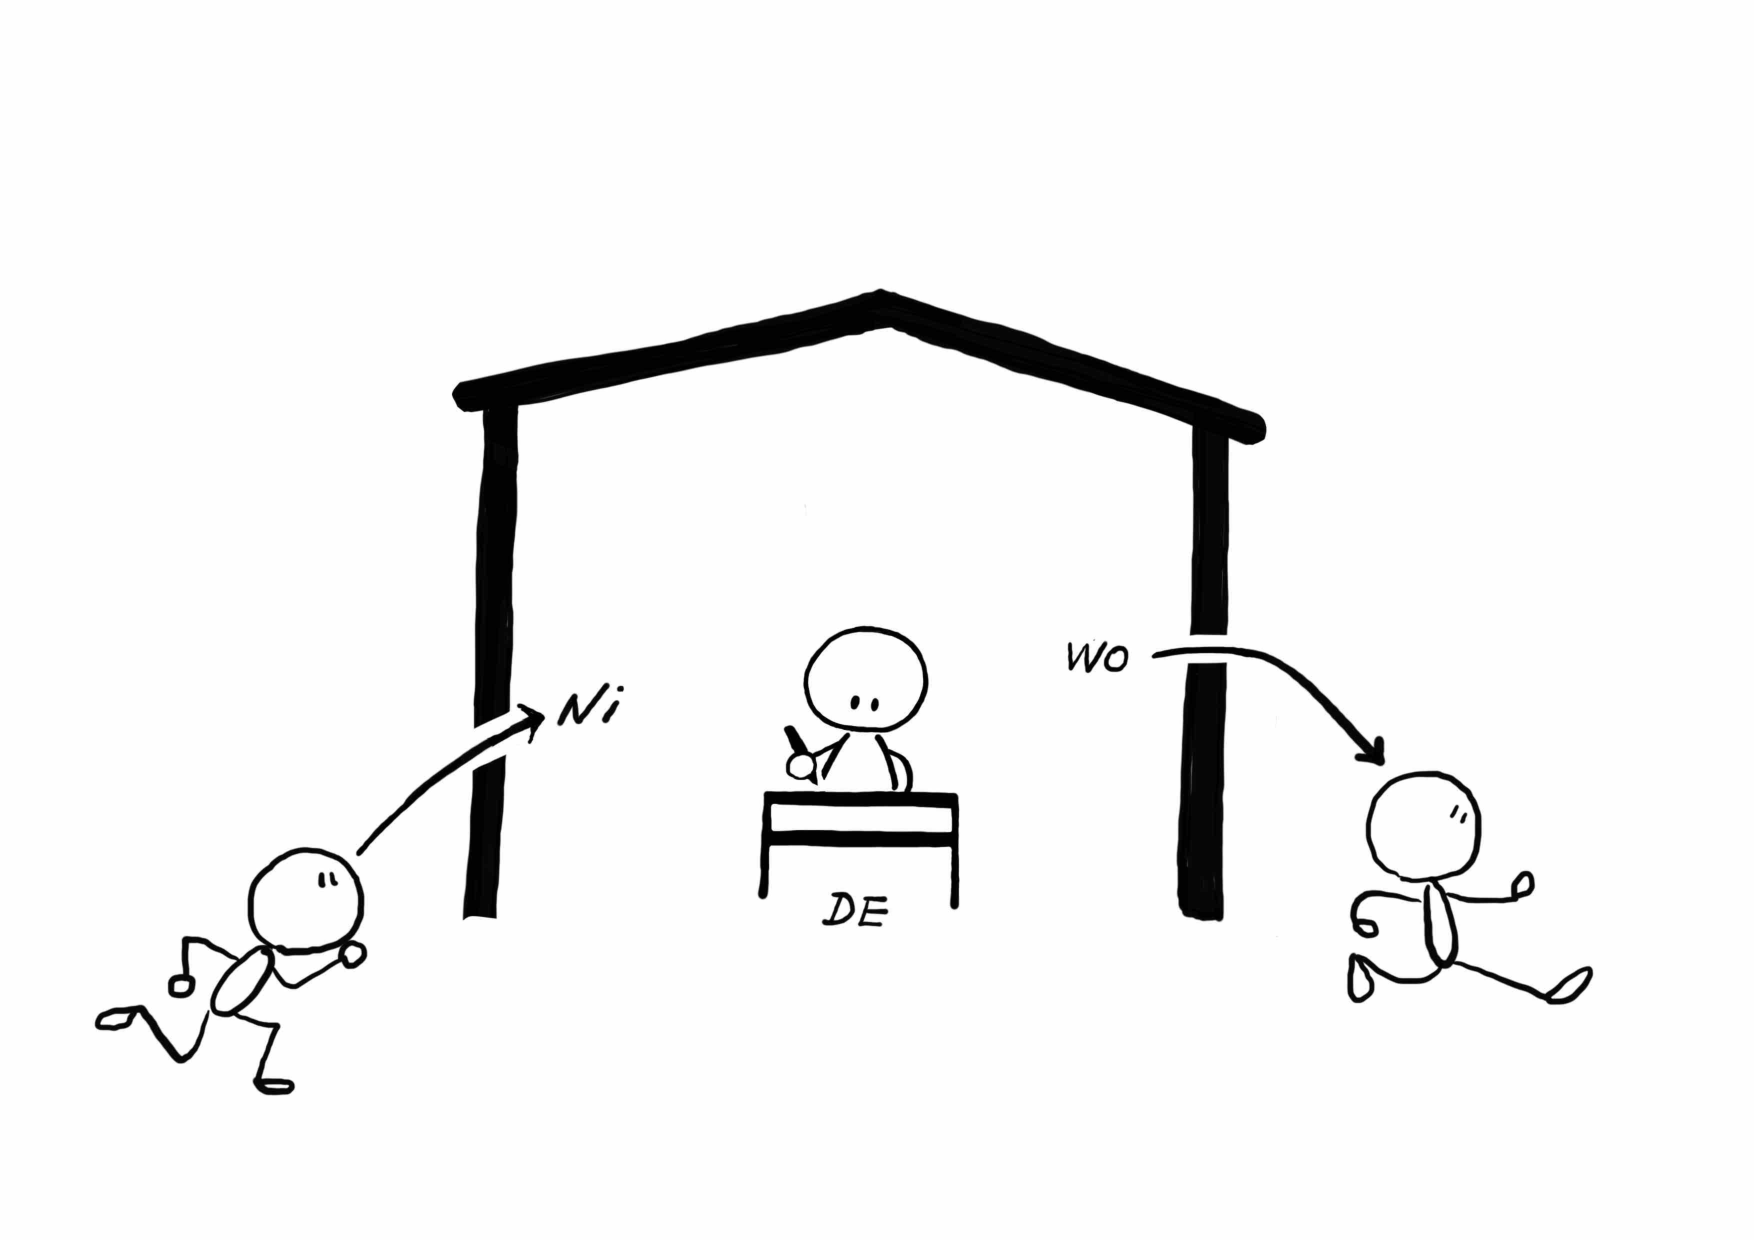
\includegraphics[trim=40 70 70 140, clip, width=.45\hsize]{toshokan-nidewo.pdf}
%\end{flushright}
%\vspace*{-0\baselineskip}

\begin{itemize}
 \item[A:] Ky\=o gogo d\=osuru? (What are you gonna do this afternoon?) 
 \item[B:] Toshokan \underline{{\bfseries de}} benky\=o. (I will study at library)
 \item[A:] Kin\=o nani shita? (Yesterday, where did you do?) 
 \item[B:] Toshokan \underline{{\bfseries de}} benkyo. (I studied at library)
 \item[A:] Jitensha de ittano? (Did you go there by bike?) 
 \item[B:] Uun, basu \underline{{\bfseries de}}. (No, by bus)
\end{itemize}

\vspace*{-1\baselineskip}

\section{Task}
 
Using a noun plus a particle style, make some sentences as short as posiblle.

\begin{multicols}{2}
\begin{enumerate}
\setcounter{enumi}{-1}   
 \item I went there by bus. $\rightarrow$  Basu de. \hrulefill
 \item \underline{\hspace*{10em}} $\rightarrow$\hrulefill
 \item \underline{\hspace*{10em}} $\rightarrow$\hrulefill
 \item \underline{\hspace*{10em}} $\rightarrow$\hrulefill
 \item \underline{\hspace*{10em}} $\rightarrow$\hrulefill
 \item \underline{\hspace*{10em}} $\rightarrow$\hrulefill
 \item \underline{\hspace*{10em}} $\rightarrow$\hrulefill
 \item \underline{\hspace*{10em}} $\rightarrow$\hrulefill
\end{enumerate}
\end{multicols}

\section{Activity}

Ask your classmates in both casual and formal style.

\begin{quote}
\begin{description}
 \item[A:] a. \underline{ Suzuki } san, gogo nani suru?
 \item[B:] b. \underline{ Toshokan de benky\=o.}
\end{description}
\end{quote}
 
\begin{enumerate}
 \item[0.]  a. \underline{ Suzuki san\hspace{6.56zw}} b. Toshokan de benky\=o.\hrulefill
 \item  a. \underline{\hspace{12zw}} b. \hrulefill
 \item  a. \underline{\hspace{12zw}} b. \hrulefill
 \item  a. \underline{\hspace{12zw}} b. \hrulefill
 \item  a. \underline{\hspace{12zw}} b. \hrulefill
 \item  a. \underline{\hspace{12zw}} b. \hrulefill
 \item  a. \underline{\hspace{12zw}} b. \hrulefill
 \item  a. \underline{\hspace{12zw}} b. \hrulefill
\end{enumerate}


\section{Review}

Fill in the blanks with particles.

\begin{enumerate}
 \item A: Ashita Doko? B: Ashita 3 ji ni daigaku \underline{\hspace{4em}}!
 \item A: Doko \underline{\hspace{4em}} iku? B: Shibuya.
 \item A: Nani \underline{\hspace{4em}} taberu? B: Onigiri mittsu.
\end{enumerate}

\ifQR
\vspace*{-6\baselineskip}
\begin{flushright}
Homework submission \includegraphics[width=24mm]{qr20180412strategic.eps}
\end{flushright}
\fi%QR

\end{document}
